\section{Available data sets}\label{sec:available-data-sets}
For the classification and localization of insects in images, an existing data set was used and extended with Bounding Box annotations.
Additionally, a cropped version of this annotated data set is created, that will be used later for the training of a \textbf{two-stage-method}.
The following section will describe the taxonomy used for the classification task, introduce used data sets
and explain what has been done to generate additional labels for the task of Bounding Box prediction.\\
It should be noted here that all image examples used for illustration in this paper have been published as part of the "\nameref{subsec:inaturalist}" data set under the \textbf{C}reative \textbf{C}ommons (CC) license, and wherever it was possible to research the origin of the images, reference has been made to the creators.

\begin{figure}[!ht]
\centering
%\hspace{2cm}
\begin{minipage}{.45\textwidth}
\vspace{1.2cm}
\centering
    \begin{tikzpicture}
    \Vertex[y=5,Pseudo]{A}\Text[y=5]{Class (Insecta)}
    \Vertex[y=4,Pseudo]{B}\Text[y=4,RGB,style={draw,color=green}]{Order (Odonata)}
    \Vertex[y=3,Pseudo]{C}\Text[y=3]{Sub-Order (Anisoptera)}
    \Vertex[y=2,Pseudo]{D}\Text[y=2]{Family (Aeshnidae)}
    \Vertex[y=1,Pseudo]{E}\Text[y=1]{Genus (Boyeria)}
    \Vertex[y=0,Pseudo]{F}\Text[y=0]{Species (Boyeria vinosa)}

    \Edge[Direct](A)(B)
    \Edge[Direct](B)(C)
    \Edge[Direct](C)(D)
    \Edge[Direct](D)(E)
    \Edge[Direct](E)(F)

    \end{tikzpicture}
    \caption{Simplified taxonomic tree of insects.
From top to bottom the tree becomes more and more fine-grained.}
    \label{fig:taxonomy}

\end{minipage}
\hfill
\begin{minipage}{.45\textwidth}

    \includegraphics[width=\textwidth]{src/images/hymenoptera-representation.eps}
    \caption{
    Samples for two families of the order Hymenoptera, compared to members of other orders.
    }
    \label{fig:hymenoptera-families}
\end{minipage}
\end{figure}
\subsection{Taxonomy}\label{subsec:taxonomy}
In order to classify objects, a general understanding of their taxonomy is required.
A taxonomy is a hierarchical scheme used for classification, that originated from categorisation of organisms.
Generally, a taxonomy includes description, identification, nomenclature and classification of groups of objects that share the same characteristic features~\cite{taxonomy}.
This taxonomy represents the underlying classes learned by the classification algorithm.
A simplified taxonomic tree for insect classification can be found in \figref{fig:taxonomy}.
This paper focuses on the detection of five "Orders" of insects that are "Coleoptera" (beetles, \figref{fig:coleoptera-sample}), "Lepidoptera" (butterflies, \figref{fig:lepidoptera-sample}), "Hemiptera" (true bugs, \figref{fig:hemiptera-sample}), "Odonata" (dragon flies, \figref{fig:odonata-sample}) and "Hymenoptera".
To simplify the detection of the order "Hymenoptera" the family "Formicidae" (ants, \figref{fig:hymenoptera-sample}) was selected.
This simplification was done, because some Hymenopteras look similar to other orders to the human eye. This would cause issues in the classification task, i.e. the order Hymenoptera contains a wide variety of differently structured and sized insects ranging from ants to wasps as sampled in \figref{fig:hymenoptera-families}.

\subsection{iNaturalist}\label{subsec:inaturalist}
The iNaturalist Species Classification and Detection Dataset (iNat data set) is a collection of image files in combination with their class labels.
It is a CVPR~\footnote{Conference on \textbf{C}omputer \textbf{V}ision and \textbf{P}attern \textbf{R}ecognition hosted by the Computer Vision Foundation (\url{https://www.thecvf.com/}} competition data set from 2021 and was originally build in 2017 with the objective to represent the unpredictable distribution of nature in regards to species and abundance~\cite{iNat}.
\subsubsection{Data set definition}
The full 2021 data set consists of approximately 2.8M images of 10,000 different species with annotated class labels~\cite{iNat-2021}.
In contrast to the original 2017 data set, the 2021 competition data does not contain annotations for Bounding Boxes.
2.7M of the image samples are combined into the public training and 100,000 into the public validation set.
The public training set data set is intended to be used during the training phase of an ML Model, which will be discussed in a later section (\ref{subsec:training-algorithms}).
The validation set is used to validate the predictive power of the current Model during this training phase.
In total, the data set contains 2,526 individual species of the class "Insecta".
It is organized in a directory structure, were directories are named by a unique identifier (UID) for each species and its taxonomic name, e.g. \path{02420_Animalia_Arthropoda_Insecta_Odonata_Euphaeidae_Euphaea_formosa}.
These directories hold the image files.
All files are in \textit{JPEG} file format and range from 6,0 kB to 105 kB in file size.
The data set was collected based on data available on the website iNaturalist.org~\footnote{iNaturalist website: \url{https://www.inaturalist.org/}}.
iNaturalist is a citizen science effort, every person can register on the website and publish or edit observations.
This means either uploading images or labeling existing images on the platform.\\
Due to the fact that not every citizen is an expert in biology, specifically in the taxonomy of \textit{all} organisms, it is presumable that the annotation data contains inaccurate species labels, albeit the data set has been reviewed by multiple citizen scientists.
Due to the power of the numbers involved, it is nearly impossible to have a 100\% accurate set of labels for almost 3M images.
By only considering the scale, for every image there is a big chance of choosing a wrong species label.
Similar, the probability of selecting a wrong species label for the insects order is considered high, as mentioned in "\nameref{subsec:taxonomy}".
But for the purpose of this work, it can be assumed that the order specification is in fact accurate, based on the argument that the species taxonomy is more fine grained than the order taxonomy and therefore harder to apply.\\
The base data set used in this project is a reduced form of the original \textit{iNat} public training data set that was provided by the team of \textit{KInsecta}.
It is prefiltered by the the taxonomic class type "Insecta", insects.
This base data set is hosted on a \textbf{N}etwork \textbf{A}ttached \textbf{S}torage (NAS) device that runs in the local network of BHT.
\begin{figure}[!ht]
    \centering
    \includegraphics[width=.80\textwidth]{src/images/image-example.eps}
    \caption{Image channels individually and combined. All channels combined result in the original image.}
    \label{fig:image-example}
\end{figure}
\subsubsection{Image data format}\label{subsubsec:data-format}
Image files can vary significantly in file formats, file size and image aspect ratios.
The here used images are in JPEG format and therefore have three channels.
Let $I \in \R^{h\times w\times 3}$ be an image of height $h$, width $w$ and with three channels, then a pixel within this image can be described as the vector $\mybold{p}\in C^{3}$, for \path{uint8} data format with $C_{\text{\path{uint8}}} = [0, 255]$.
When loaded the values are converted to \path{float32} with $C_{\text{\path{float32}}} = [0, 1]$.
Each of the elements of $\mybold{p}$ represent a color intensity for the corresponding channel.
The three channels are a \textbf{R}ed, a \textbf{G}reen and a \textbf{B}lue channel.
To recreate the image the channels are combined in their spacial dimension (\figref{fig:image-example}),
\begin{align}
    I = [R_I, G_I, B_I]
\end{align}
where $R_I, G_I$ and $B_I$ are the corresponding color-channel-element-$h \times w \times 1$-matrices with $h$ rows and $w$ columns respectively.\\
This simplifies working with images drastically, as they can be interpreted and used as a matrix.
Due to this format a single pixel can easily be queried using its coordinates in the image $P = I(x, y)$, or e.g. $P_R = R_I(x, y)$ for the corresponding red value of this pixel.
In the following, the computer vision (CV) notation of $P = I(y, x); P_R = R_I(y, x)$ will be used.
This is a notation simplified for the image data format and is introduced in this context due to the way the data is stored on the computer: as an array, which is accessed by its height component first, e.g. \path{image[height][width]}.
Additionally, the underlying coordinate system is a down-right positive Cartesian coordinate system, ranging from the origin, the top left corner of the image to the lower right corner.\\
Apart from the information stored in each pixel, a second important information is the height and width of the image.
In order to process images further and to feed them into the Machine Learning algorithms mentioned earlier, the images need to be rescaled into a unified size.
The size was fixed here at $224px\times224px$~\footnote{The scale $224px\times224px$ was used in the VGG-16 paper and was here adopted to achieve best results with this architecture.}.
For scaling purposes in this project the bilinear interpolation method is used, which is a two dimensional variant of linear interpolation and the default configuration of most Tensorflow methods~\footnote{Tensorflow documentation for the image resizing function: \url{https://www.tensorflow.org/api_docs/python/tf/image/resize}}.
An interpolation method was selected in order to not change the information in the input features.
Filling the images with black pixels to maintain the original image aspect ratio, but artificially add more content to it, would add additional information to the input features and would distort the results.
\subsection{Collection}\label{sub:collection}
As previously mentioned, the base data set ${iNat_{\text{train}}}_{Insecta}$ is only a subset of the original \textit{iNat}-2021 data set $iNat$.
It contains 663,682 image files scattered unbalanced across 2527 insect species.
The data set extracted for the experiments $X$ is an evenly distributed subset of the nearly 660,000 insect image files and contains 500 samples per order.
A simplified visualization of this set substitution can be found in \figref{fig:dataset-venn}.\\
To reduce network traffic and prevent issues with connecting to the \textit{NAS} server, some precocious preparations were made, i.e. the data collection pipeline, one of the Python script files in the accommodating repository of this paper, was developed on a very reduced subset, five pictures, of the overall data set.
The script allows random selection of $n$ species per order and $m$ samples for each of them by providing the desired parameters accordingly.
A storage directory is created as a temporary storage directory for simplified usage during "\nameref{subsec:manual-labeling}"
and was required to solve the issue of changed file paths during the upload phase into the labeling tool.

\begin{figure}[!ht]
    \centering

    \begin{tikzpicture}

        % Set A
        \node [draw,
            ellipse,
            minimum width =5cm,
            minimum height=2.5cm,
            fill=lightgray] (A) at (0,0){};

        % Set B
        \node [draw,
            ellipse,
            minimum width =4cm,
            minimum height=2cm,
            fill=CornflowerBlue] (B) at (0.5,0){};

        \node [draw,
            ellipse,
            minimum width =2.5cm,
            minimum height=1.75cm,
            fill=YellowGreen] (C) at (1.25,0){};

        \node [draw,
            ellipse,
            minimum width =0.5cm,
            minimum height=0.25cm,
            fill=BurntOrange] (D) at (2,0) {};

        \node[] (Al) at (-2, 0){$iNat$};
        \node[] (Bl) at (-0.7, 0){$iNat_{\text{train}}$};
        \node[] (Cl) at (3.5, -0.75){${iNat_{\text{train}}}_{Insecta}$};
        \node[] (Dl) at (3, 0.75){$X$};

        \draw[-latex] (Dl) -- (D.center);
        \draw[-latex] (Cl) -- (1.5, -0.5);
    \end{tikzpicture}

    \caption{Venn diagram of the used data sets $DS\subset {iNat_{\text{train}}}_{Insecta} \subset iNat_{\text{train}} \subset iNat$, where $X$ is the data set used in this project.}
    \label{fig:dataset-venn}
\end{figure}


\begin{comment}
\subsection{[DEPRECATED] \textit{KInsekt}-Project}\label{subsec:textit{kinsekt}-project}
\subsection{Hand-drawn sketches}\label{subsec:hand-drawn-sketches}
TBD (to be discussed)

A second data set was provided from another Bachelor's student working in the \textit{KInsecta} team.
This data set consists of 726 hand drawn sketches,
containing 156 images of Hymenoptera-Formicidae (\lstinline{01-Ameisen})
140 images of class Odonata (\lstinline{02-Libellen}),
120 images of class Coleoptera (\lstinline{03-Marienkaefer}),
190 images of class Lepidoptera (\lstinline{04-Schmetterlinge}) and
120 images of class Hemiptera (\lstinline{05-Wanze})

\end{comment}

\subsection{Manual labeling}\label{subsec:manual-labeling}
For the localization task of this paper an extended data set containing locations of insects, in each image, is required.
As representation for these locations Bounding Boxes (BBs) are used.
BBs are rectangular boxes, a subset of pixels of the original image, that contain an object.
Each BB is represented as coordination vector in the form
\begin{align}
    \mybold{c^{(m)}} =
    \left(
        y^{(m)}_{\min},
        x^{(m)}_{\min},
        h^{(m)},
        w^{(m)}
    \right)^T
    \label{eq:bb}
\end{align}
where $y^{(m)}_{\min}$ and $x^{(m)}_{\min}$ are the coordinates of the upper-left corner of the $m$-th BB in a data set, and $h^{(m)}$ and $w^{(m)}$ height and width respectively.
This turned out to be less error prone in further usage~\footnote{
    A more detailed description will follow in the section "\nameref{subsec:roadblocks}".
}.
In order to make the annotated BBs available for later use in the \textit{KInsecta} team \href{https://labelstud.io/}{LabelStudio}~\cite{Label-Studio} was used.
LabelStudio is a self hosted open source labelling tool managed by \textit{KInsecta} within the BHT.
Using LabelStudio the data set of the 2500 pre-selected \textit{iNat} image files was manually labelled.
\figref{fig:label-studio-1} gives an overview on how the interface of Label Studio looks like.
\begin{wrapfigure}{l}{.45\linewidth}
    \centering
    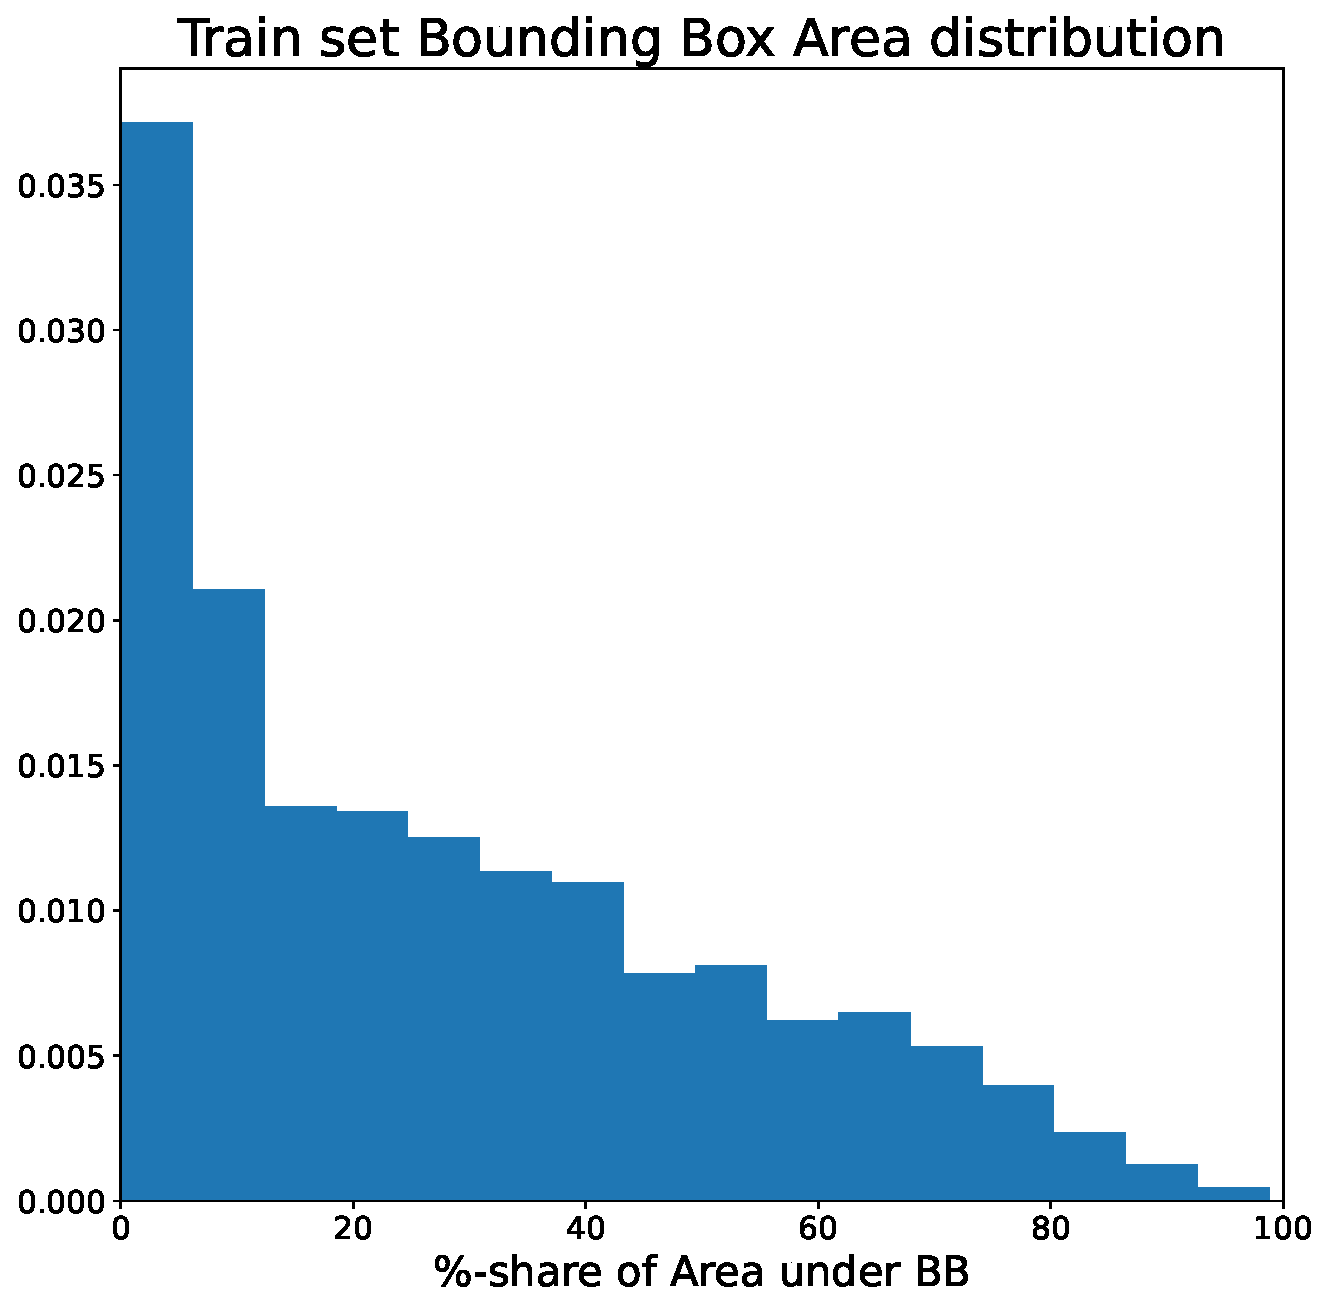
\includegraphics[width=.45\textwidth]{src/images/bounding-box-area-distribution.eps}
    \caption{Distribution of share of area under BBs.}
    \label{fig:bb-area-distribution}
\end{wrapfigure}
The BBs can be exported from LabelStudio in JSON file format and are stored in a dictionary-like fashion, where each image file is linked to the manually created BB annotations.
An example for the representation can be seen in "\nameref{A1}".
In order to get an understanding of the manually generated data a final area distribution for the created BBs can be seen in \figref{fig:bb-area-distribution}.
This will be useful for the following section, in which the data gets preprocessed, augmented and wrapped into a final data set, that is used for the rest of the project.

\vfill
\begin{figure}[!ht]
    \centering
    \includegraphics[width=\textwidth]{src/images/LS-2.png}
    \caption{Annotation-View of LabelStudio: Bounding Boxes can be selected using Drag\&Drop mechanics; Each BB is labelled with a corresponding order-label.}
    \label{fig:label-studio-1}
\end{figure}
